\section{Hardware Assembly and Circuit Diagram}
{\fontsize{12}{14}\selectfont
        \begin{figure}[H]
            \centering
            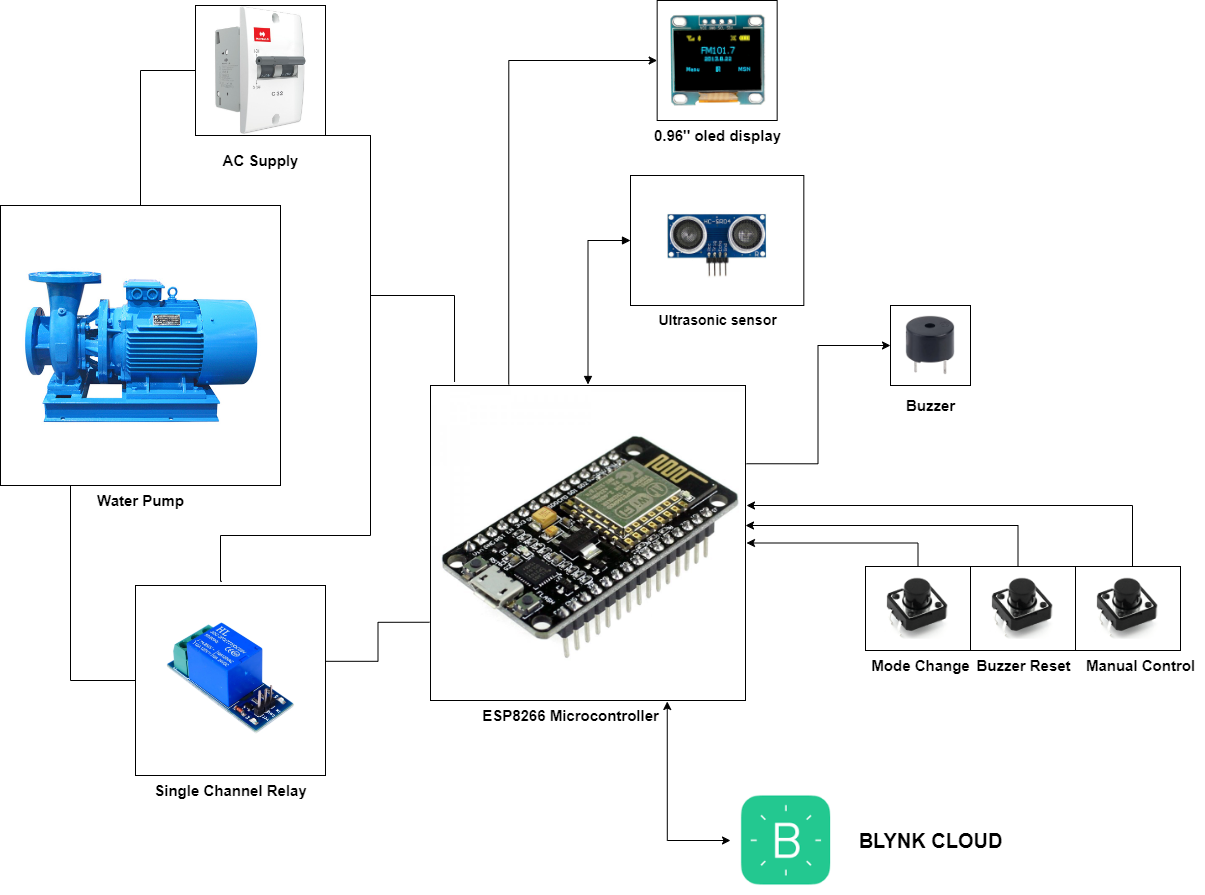
\includegraphics[width=6in]{diagram.png} \\
            \caption{Water Level Monitoring and Control Circuit Diagram}
            \label{fig:diagram} % Optional: for referencing
        \end{figure}

The hardware setup of this IoT-based water level monitoring and pump control system integrates multiple components to ensure real-time data acquisition, remote monitoring, and automated control of the water pump. \\
\newpage
\noindent
The following components are used in the system, with each playing a crucial role: \\
\begin{enumerate}
  \item \textbf{ESP8266 Microcontroller}\\
The ESP8266 is the core of the system, acting as the main controller for processing data from sensors, controlling output devices, and managing communication with the Blynk cloud platform. Its built-in Wi-Fi module allows seamless remote monitoring and control via the Blynk mobile application.

  \item \textbf{Ultrasonic Sensor (HC-SR04)}\\
The HC-SR04 ultrasonic sensor measures the distance between itself and the water surface, determining the water level in the tank. It sends high-frequency sound waves and calculates the time taken for the echo to return, which the ESP8266 processes to derive the water level.
  
  \item \textbf{0.96" OLED Display}\\
The OLED screen provides a local, real-time display of the water level. It serves as an immediate visual representation of the tank's status for users near the system.

  \item \textbf{Single Channel Relay Module}\\
The relay acts as a switch to control the water pump. Based on the water level thresholds processed by the ESP8266, the relay automatically activates or deactivates the water pump.

  \item \textbf{Water Pump}\\
The water pump fills the tank when the water level is low. Its operation is automated by the ESP8266 via the relay module.

  \item \textbf{Push Buttons}\\
    Three push buttons provide manual control and additional functionality:
    \begin{itemize}
      \item \textbf{Mode Change Button:} Toggles between different operational modes, such as automatic and manual control.
      \item \textbf{Buzzer Reset Button:} Silences the buzzer when a critical water level alert is triggered.
      \item \textbf{Manual Control Button:} Allows the user to turn the pump on or off manually.
    \end{itemize}

  \item \textbf{Buzzer}\\
The buzzer provides an audible alert for critical conditions, such as the tank being nearly empty or full. It ensures users are immediately aware of the system's status.

  \item \textbf{AC Power Supply}\\
The water pump is powered by an AC power supply, with the system ensuring safe and efficient operation.
\end{enumerate}

\noindent
\textbf{Circuit Diagram Explanation}\\
The circuit diagram visually represents the interconnections between the various hardware components. Each component is linked to the ESP8266, forming a centralized control system.
\noindent
The HC-SR04 ultrasonic sensor is connected to the ESP8266 via its trigger and echo pins. These signals are processed to determine the water level in the tank.
The OLED display communicates with the ESP8266 through an I2C interface to show real-time water level data.
The relay module connects to the ESP8266’s GPIO pins to control the water pump based on the processed data.
The push buttons are connected to the GPIO pins of the ESP8266, enabling manual user input for operational adjustments.
The buzzer is connected to another GPIO pin and is activated for critical alerts.
The ESP8266 sends data to the Blynk cloud platform via its Wi-Fi module, enabling remote monitoring and control through a smartphone app.
System Functionality
The ultrasonic sensor continuously monitors the water level and sends data to the ESP8266 for processing.
Based on predefined thresholds, the ESP8266 decides whether to turn the water pump on or off.
Data is displayed locally on the OLED screen and transmitted to the Blynk cloud for remote monitoring.
The push buttons allow users to override the system for manual control, reset alarms, or switch between modes.
Alerts are triggered via the buzzer and mobile notifications for low or critical water levels.
This circuit diagram reflects the modular and scalable nature of the system, making it suitable for future enhancements, such as additional sensors or water quality monitoring modules.

\section{Software Development and Integration with Arduino IDE and Blynk}
The software development process forms the backbone of the water monitoring and control system, enabling seamless communication between hardware components, real-time monitoring, and remote control functionality. The system leverages the Arduino IDE for microcontroller programming and the Blynk platform for IoT integration, creating a robust and user-friendly solution. This section provides a detailed explanation of the software design and implementation, highlighting its key components and functionalities.\\

\subsection{Arduino IDE Setup and Programming}
The Arduino IDE serves as the primary environment for programming the ESP8266 microcontroller. It provides tools for writing, debugging, and uploading code, ensuring efficient interaction with the system's hardware components.
\begin{enumerate}
  \item \textbf{Environment Setup:}\\
    \begin{itemize}
      \item The Arduino IDE is configured to support the ESP8266 microcontroller by adding the ESP8266 board manager through the IDE preferences. This allows seamless compatibility between the IDE and the hardware.
      \item Relevant drivers are installed to ensure the microcontroller is recognized by the computer.
    \end{itemize}
  \item \textbf{Library Installation:}
    \begin{itemize}
      \item Essential libraries are integrated into the IDE to enable specific functionalities:
      \begin{itemize}
        \item Blynk Library: Facilitates communication between the ESP8266 and the Blynk cloud platform.
        \item Adafruit GFX and SSD1306 Libraries: Support the OLED display module for real-time data visualization.
        \item Ultrasonic Sensor Library: Simplifies the interaction with the HC-SR04 ultrasonic sensor.
      \end{itemize}
      \item These libraries are added through the library manager or manually imported into the project.
    \end{itemize}
  \item \textbf{Code Development:}
    The software is designed to handle multiple tasks simultaneously, ensuring the system operates efficiently. Key code components include:
    \begin{itemize}
      \item \textbf{Sensor Data Acquisition:}\\
        The HC-SR04 ultrasonic sensor measures the water level by calculating the distance between the sensor and the water surface. The sensor's echo and trigger pins are defined, and the data is read using precise timing functions.
      \item \textbf{Data Processing:}\\
        The raw sensor data is processed into meaningful water level values, which are then used to determine system actions. For instance, threshold levels are set to activate or deactivate the water pump.
      \item \textbf{OLED Display Control:}\\
        The processed water level data is sent to the OLED display for local visualization. The display updates in real-time to provide an intuitive interface for users.
    
      \item \textbf{Buzzer Alerts:}\\
        The buzzer is activated when critical water levels are reached, providing an audible alert to ensure timely action.
    
      \item \textbf{Automation Logic:}\\
        Control logic is implemented to automatically switch the water pump on or off based on water level thresholds. This reduces the need for manual intervention.
    \end{itemize}
    \item \textbf{Testing and Debugging:}
    The Arduino IDE’s serial monitor is utilized extensively during development to monitor real-time data from the microcontroller. Debugging tools within the IDE help identify and resolve any issues in the code, ensuring smooth operation.
\end{enumerate}

\subsection{Blynk Cloud Integration}
Blynk is employed as the IoT platform to enable real-time monitoring and remote control through a mobile application. It acts as a bridge between the ESP8266 microcontroller and the user, providing an intuitive interface for system management.
\begin{enumerate}
  \item \textbf{Cloud Platform Configuration:}\\
    A Blynk account is created, and a new project is set up within the mobile application.
    An authentication token generated by Blynk is included in the Arduino code, linking the microcontroller to the cloud platform.
  \item \textbf{Wi-Fi Connectivity:}\\
    The ESP8266 is programmed to connect to a Wi-Fi network using the SSID and password provided in the code. This connection enables the microcontroller to send and receive data via the Blynk cloud.
  \item \textbf{Mobile Application Widgets:}\\
    The Blynk mobile application is configured with various widgets to enhance user interaction:
    \begin{itemize}
      \item Value Display: Displays the current water level in real-time.
      \item Button Widget: Allows manual control of the water pump.
      \item Gauge Widget: Provides a graphical representation of the water level.
      \item Notification Widget: Sends alerts to the user’s mobile device for critical events, such as low or high water levels.
    \end{itemize}
  \item \textbf{Data Transmission:}
    \begin{itemize}
      \item The processed water level data from the ultrasonic sensor is transmitted to the Blynk cloud via virtual pins.
      \item The Blynk platform relays this data to the mobile application, where users can monitor it in real-time.
    \end{itemize}
  \item \textbf{Control Mechanisms:}
    \begin{itemize}
      \item Users can control the water pump remotely through the Blynk app.
      \item Manual overrides are supported, allowing users to activate or deactivate the pump as needed, irrespective of the automation logic.
    \end{itemize}
  \item \textbf{Automation Features:}\\
    The Blynk platform integrates seamlessly with the automation logic in the Arduino code. For example, when a critical water level is reached, the system sends a notification to the user while simultaneously triggering the appropriate system response.
\end{enumerate}

\noindent
By combining Arduino IDE and Blynk, the system benefits from a simple yet powerful development and integration process. The Arduino IDE provides flexibility and control over the microcontroller, while Blynk offers user-friendly tools for IoT integration. Together, they create a system that is reliable, responsive, and accessible.\\
\noindent
This software setup allows for real-time monitoring, efficient automation, and intuitive remote control, making it a vital component of the water monitoring and control system.
}
    